\def\year{2015}
%File: formatting-instruction.tex
\documentclass[letterpaper]{article}
\usepackage{aaai}
\usepackage{times}
\usepackage{booktabs}
\usepackage{helvet}
\usepackage{courier}
\usepackage{amsmath}
\usepackage{threeparttable}
\usepackage{slashbox}
\usepackage{amssymb}
\usepackage{color}
\usepackage{graphicx}
\usepackage{subfigure}
\frenchspacing
\setlength{\pdfpagewidth}{8.5in}
\setlength{\pdfpageheight}{11in}
\pdfinfo{
/Title (PM2.5 concentration prediction using times series based data mining)
/Author (Jiaming Shen)}
\begin{document}
% The file aaai.sty is the style file for AAAI Press 
% proceedings, working notes, and technical reports.
%
\title{$\text{PM}_{2.5}$ concentration prediction using times series based data mining}
\author{Jiaming Shen\\
Shanghai Jiao Tong University, IEEE Honor Class\\
Email: mickeysjm@gmail.com\\
}
\nocopyright
\maketitle
\begin{abstract}
\begin{quote}
Prediction of particulate matter with diameter less than 2.5 $\mu$m ($\text{PM}_{2.5}$) is an important issue in control and reduction of pollutants in the air. In this report, I discuss three different models to deal with this $\text{PM}_{2.5}$ prediction problem, including basic Autoregressive Moving Average (ARMA) Model, Stochastic Volatility (SV) Model and Stock-Watson (SW) Model. Furthermore, I design an innovative model combining SW model with Time Series Neural Network. Finally, I conduct four experiments to compare and analyze the performances of above-mentioned models. The results show that this newly-designed model provide more accurate predictions of $\text{PM}_{2.5}$ concentration levels for the next six hours.
\end{quote}
\end{abstract}

%Introduction
\section{Introduction}
Particulate matter (PM) is the term used for a mixture of solid particles and liquid droplets found in the air. In particular, fine particles with diameter less than 2.5 $\mu$m are called $\text{PM}_{2.5}$. Prediction of $\text{PM}_{2.5}$ is an important issue in control and reduction of pollutants in the air. Predictive models for $\text{PM}_{2.5}$ vary from extremely simple to extremely complex, but the ability to accurately forecast $\text{PM}_{2.5}$ concentration index remains elusive. 

In this report, I discuss my effort to solve this problem using times series based data mining. I first adopt three distinctive models, including basic Autoregressive Moving Average (ARMA) Model, Stochastic Volatility (SV) Model and Stock-Watson (SW) Model. Furthermore, I design a new method combining SW model with Time Series Neural Network, adding external meteorological information such as temperature, pressure, humidity, windspeed and precipitation rate. Finally, I conduct four experiments to compare and analyze the performances of above-mentioned models, using the dataset provided by the U.S. Department of State. The results show that this newly-designed model provide more accurate predictions of $\text{PM}_{2.5}$ concentration levels for the next six hours.

The rest of this report is structured as following: In section 2, I give a thorough discussion of the dataset I used in this project. In section 3, specific task goals are presented. ARMA model, Stochastic Volatility Model, Stock-Watson Model and Stock-Watson Model with External Information are discussed in Section 4 - 7, respectively. Finally, I talk about the future works and conclude this report in Section 8.




%Dataset
\section{Dataset}
The dataset I use in this project is the U.S. Department of State air quality files [1], which contain $\text{PM}_{2.5}$ in concentration unit $\mu \text{g}/\text{m}^{3}$ from each post. Files include hourly data of following several attributes -- Site, Parameter, Dates(LST), Year, Month, Day, Hour, Value, Unit, Duration, and QC Name.  \text{Site} is the city where the measurements were taken. In this project, I only use four major cities in China, and their detail locations are shown in Table 1. \text{Value} is the measurement in concentration, and the value of missing data point is listed as -999. \text{QC Name} is the quality control status of the data; either valid or missing. Further explanations of this raw dataset file can be viewed in [2].

%%%Table 1: Geographic Coordinates for the locations of Four Major Cities
\begin{table}[h]
\begin{center}
\begin{threeparttable}
\begin{tabular}{c c}
    \toprule
    \text{Site Location} & \text{Latitude and Longitude Degrees} \\ 
    \midrule
       Shanghai  & 31.21, ~~ 121.44 \\
       Beijing   &  39.95, ~~ 116.47 \\ 
	Guangzhou   &  23.12, ~~ 113.32 \\ 
	Chengdu   &  30.63, ~~ 104.07 \\ 
      \bottomrule
\end{tabular}
\end{threeparttable}
\end{center}
\caption{Geographic Coordinates for the locations of Four Major Cities}
\end{table}

From the raw dataset files, I notice that these data have not been fully validated or quality assured, and thus they should be considered preliminary. Before conducting any further experiment, I first have a thorough look at the raw dataset, finding the number and percentage of missing data point.
The missing data point means either the Value is -999 or the QC Name is labeled ``Missing''. The results are shown in Table 2. As you can see, the percentage of missing data points of Guangzhou in Year 2014 is too high ( above 5 \%), and thus I switch to the dataset in Year 2013. Except for Guangzhou, I use the latest dataset for analyzing all other major cities, namely using the dataset in Year 2014. 

%%%Table 2: Number of Missing Data Points of Four Major Cities in Three Different Years
\begin{table}[h]
\centering
\begin{tabular}{|l||*{3}{c|}}\hline 
\backslashbox{City}{Year} 
&\makebox[3em]{2012}&\makebox[3em]{2013}&\makebox[3em]{2014} \\[0.3em]\hline\hline
Shanghai & 279 & 173 (1.97\%) & 103 (1.17\%) \\[0.3em]\hline 
Beijing & 489  & 82 (0.94\%) & 99  (1.13\%) \\[0.3em]\hline 
Chengdu  & 4370  & 1393 (15.9\%)& 285 (3.25\%) \\[0.3em]\hline 
Guangzhou & 2188 & 371 (4.23\%) & 645 (7.36\%)\\[0.3em]\hline 
\end{tabular} 
\caption{Number of Missing Data Points of Four Major Cities in Three Different Years}
\end{table}

For the sake of temporal continuity, I did not simply delete those missing data. Instead, I use first-order interpolation method to replace them, and conduct simple statistical analysis in original data set. Results are shown in Figure 1 as well as Table 3. Obviously, Beijing has the worst air condition among all four major cities in China, which is consistence with our intuition.

%%%Figure 1: Boxplot of $\text{PM}_{2.5}$ Concentration Index
\begin{figure}[htbp]
	\centerline{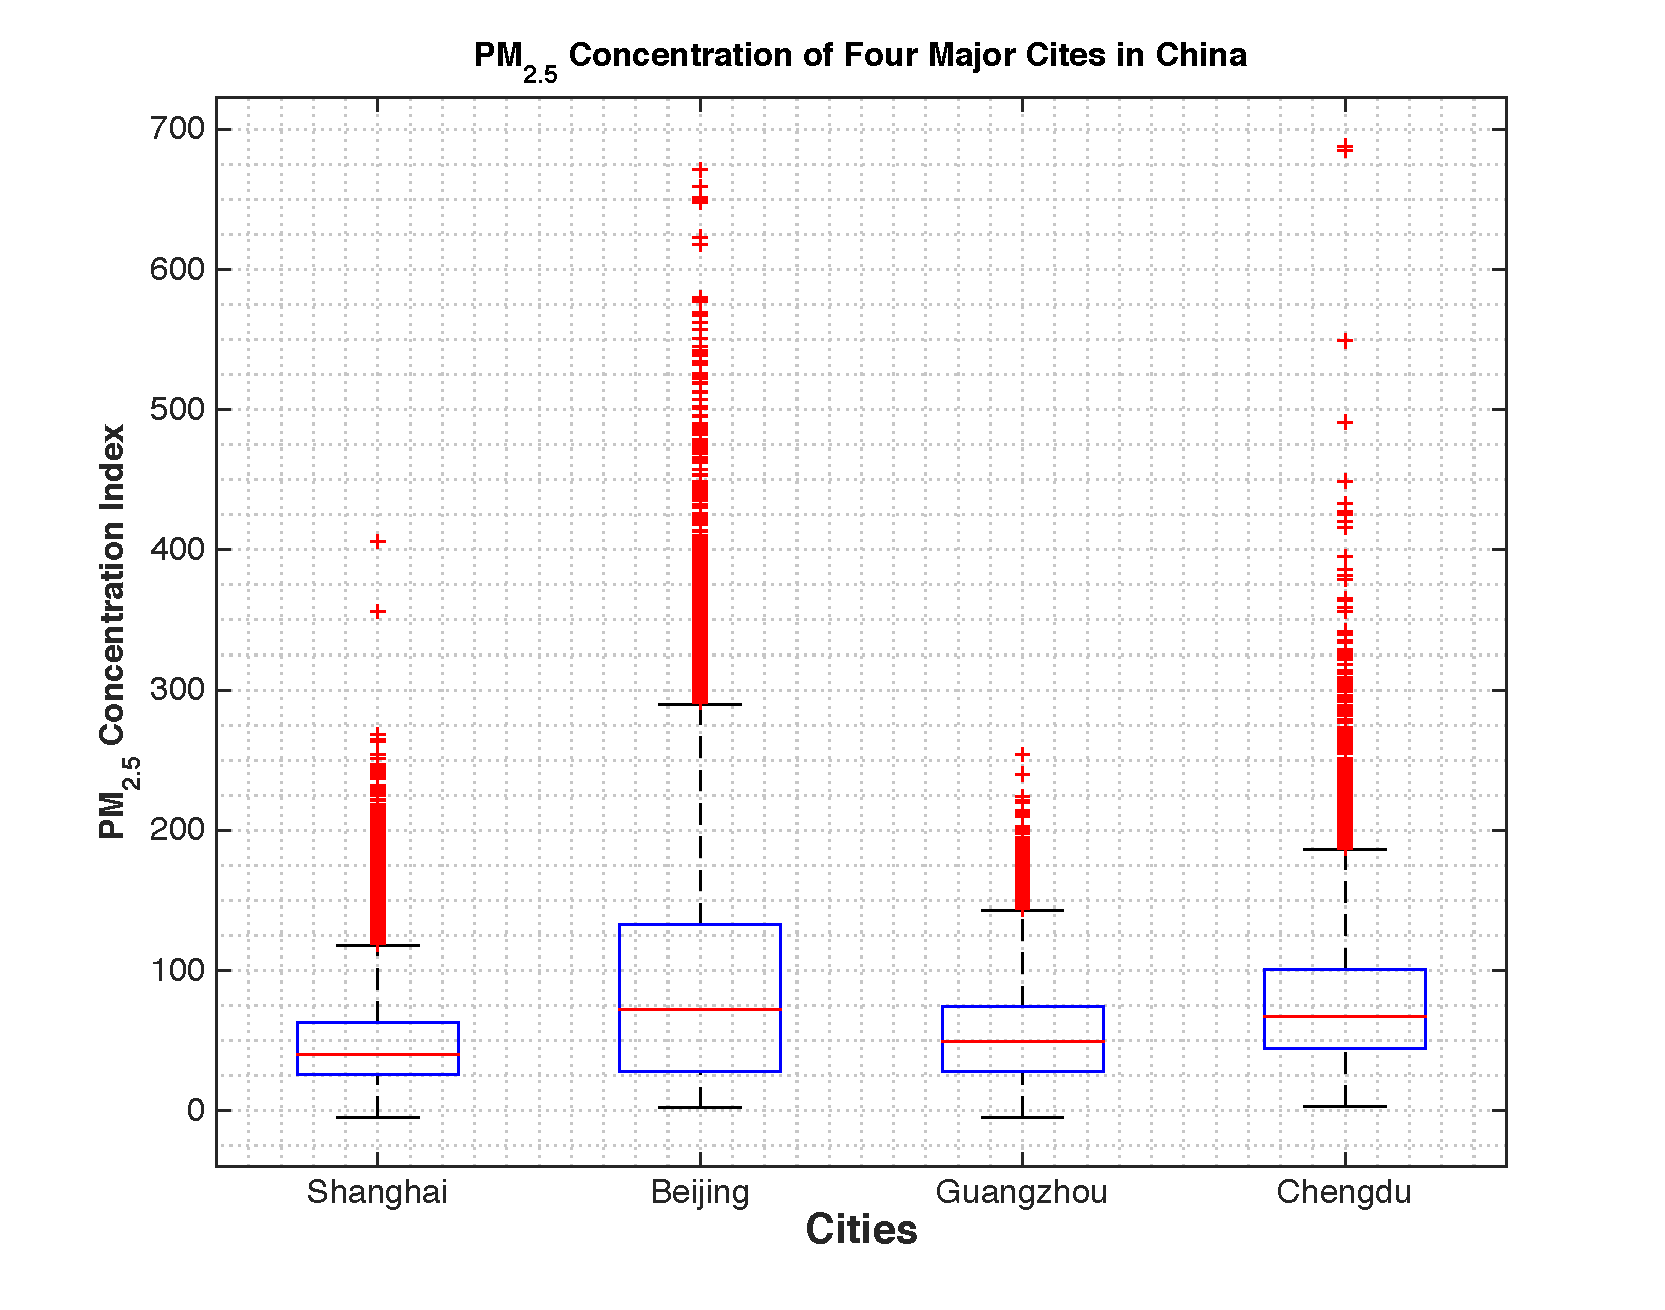
\includegraphics[width=0.50\textwidth]{PM25_values.pdf}}
	\caption{Boxplot of $\text{PM}_{2.5}$ Concentration Index}\label{fig:digit}
\end{figure}

%%%Table 3: Statistics of $\text{PM}_{2.5}$ Concentration Index
\begin{table}[h]
\centering
\begin{tabular}{|l||*{3}{c|}}\hline 
\backslashbox{City}{Statistics} 
&\makebox[2.4em]{Mean}&\makebox[7em]{Standard Deviation}&\makebox[2.4em]{Median} \\[0.3em]\hline\hline
Shanghai & 49.54 & 36.03 & 40 \\[0.3em]\hline 
Beijing & 97.95 & 93.83 & 72 \\[0.3em]\hline 
Guangzhou & 55.15 & 34.72 & 49\\[0.3em]\hline 
Chengdu  & 81.06 & 54.09 & 67 \\[0.3em]\hline 
\end{tabular} 
\caption{Statistics of $\text{PM}_{2.5}$ Concentration Index}
\end{table}

Perhaps, you do not have an intuitive understanding of what the $\text{PM}_{2.5}$ concentration index means exactly. You can find a basic Air Quality Guide for $\text{PM}_{2.5}$ in [1]. Here, in Figure 2, I want to show you the $\text{PM}_{2.5}$ concentration index of different status in four major cites of China. As you can see, the air qualities in over 50 days are labelled ``Unhealthy for Sensitive Group'' in Beijing and there are another 50 days are considered ``Unhealthy'' and ``Very Unhealthy''. The situation better is Shanghai, but there are still about 20 days with air qualities labelled ``Unhealthy for Sensitive Group''. These astonishing facts further strengthen the motivation of analyzing $\text{PM}_{2.5}$ concentration in China.

%%%Figure 2: \text{PM}_{2.5}$ of different status in four major cites of China
\begin{figure}[htbp]
	\centerline{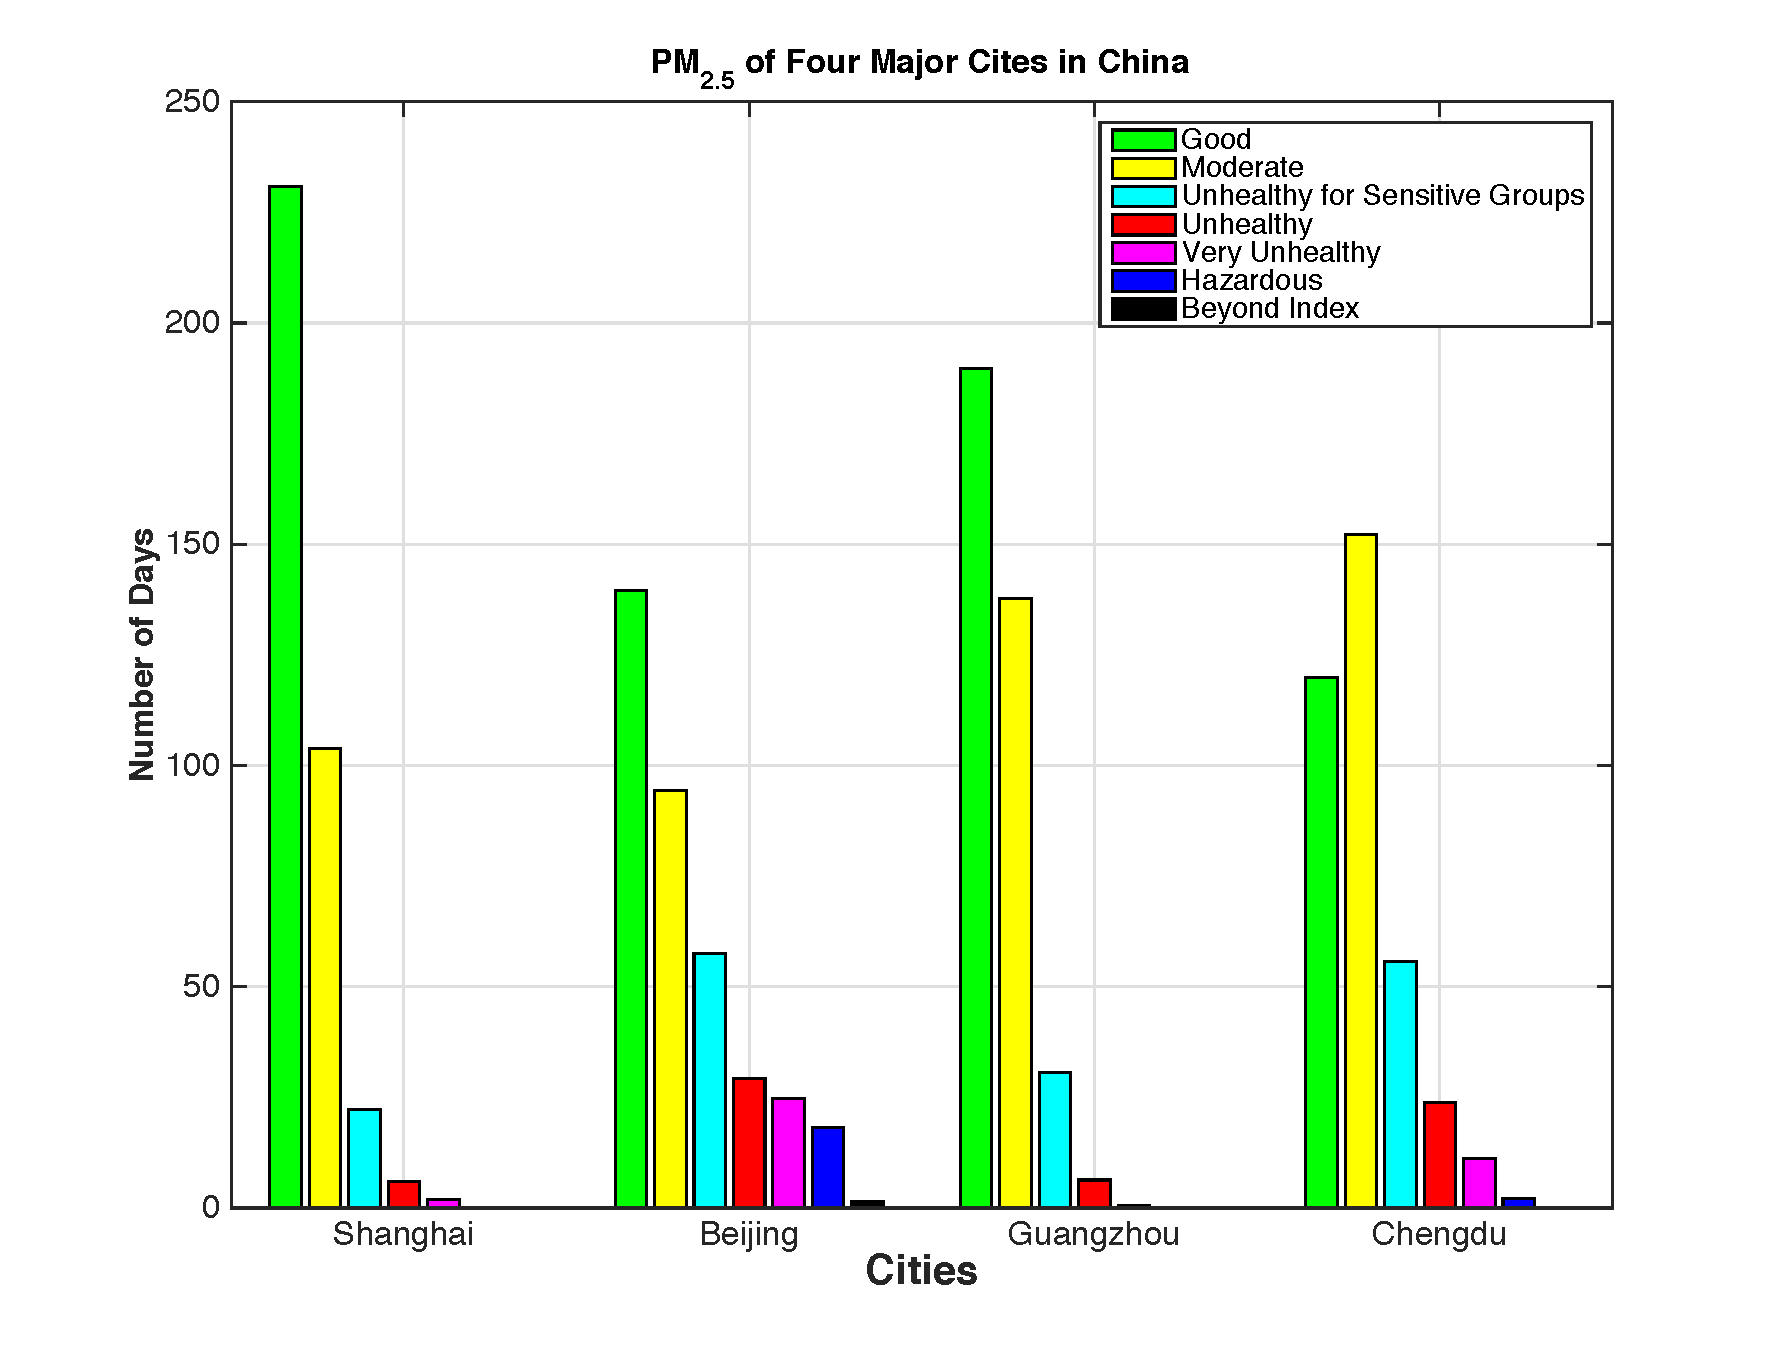
\includegraphics[width=0.55\textwidth]{PM25_days.pdf}}
	\caption{$\text{PM}_{2.5}$ of different status in four major cites of China}\label{fig:digit}
\end{figure}

%Task Goals
\section{Task Goals}
As I do not have a specific task goal in the original version of this project, I need to define them on my own. Actually, good task goals serve not only the purpose of conducting this project, but also decide whether this project is meaningful at all. Good task goals should be both intuitive and profound; they requires deep understandings of the whole problem and point out the direction I will be working on. In this project, I establish three different categories of task goals, namely \textbf{$\text{PM}_{2.5}$ Trend Prediction}, \textbf{$\text{PM}_{2.5}$ Value Prediction}, and \textbf{$\text{PM}_{2.5}$ Hidden Factors Prediction}. They will be discussed detailedly in following three subsections.

\subsection{$\text{PM}_{2.5}$ Trend Prediction}
Given a sequence of historical $\text{PM}_{2.5}$ data, we want to predict whether the following six hour's $\text{PM}_{2.5}$ concentration indexes will increase, decrease or basically stay stable. This is call $\text{PM}_{2.5}$ Trend Prediction, which is the most basic task goal of our project. 

\subsection{$\text{PM}_{2.5}$ Value Prediction}
Given a sequence of historical $\text{PM}_{2.5}$ data, we want to predict the exact value of $\text{PM}_{2.5}$ concentration indexes in next one or several time units. This is an advanced version of $\text{PM}_{2.5}$ Trend Prediction problem. Besides, if we only predict one time unit ahead, we call it \text{One step ahead prediction}, or if we want to predict several time units ahead, we call it \text{Multiple steps ahead prediction}. Obviously, the later one is a more challenging problem and require more complex model to solve it. Finally, we should pay attention to the usage of ``time unit''. The raw dataset provides hourly $\text{PM}_{2.5}$ concentration index, so intuitively the time unit could be ``Hour''. We can see aggregate these values and change the ``time unit'' to be ``Every Six Hour'', or simply ``Day''. Here, in this project, I DO NOT change the time unit, and keep using ``Hour'' as the basic and single ``time unit'', however, we can modify this in future works, for some other specific problems.

\subsection{$\text{PM}_{2.5}$ Hidden Factors Prediction}
Given a sequence of historical $\text{PM}_{2.5}$ data, we want to evaluate and predict the hidden factors which generate or influence the observable $\text{PM}_{2.5}$ concentration indexes. This is called $\text{PM}_{2.5}$ Hidden Factors Prediction, which is a higher level of prediction because it not only shows us the facts (observable $\text{PM}_{2.5} concentration indexes$ ) on surface, but also analyzes the reasons in deeper level, i.e. hidden factors.

%Experiment: ARMA Model
\section{Experiment I: ARMA Model}
The first model I used to achieve the task goals in previous section is Autoregressive Moving Average (ARMA) Model. The fundamental assumption of the model is that the value of the series at time $t$, $X_{t}$, \textbf{linearly} depends on its previous $p$ values (deterministic part) and on a random disturbance $\tilde{Z_{t}}$ (stochastic part). We can write

\begin{displaymath}
X_{t} = \phi_{1} X_{t-1} + \phi_{2} X_{t-2} + \cdots + \phi_{p} X_{t-p} + \tilde{Z_{t}},
\end{displaymath} 

\noindent where $\{ \phi_{1}, \phi_{2}, \cdots, \phi_{p} \}$ are real constants called \emph{autoregressive (AR) coefficients}. $\tilde{Z_{t}}$ is the disturbance at time $t$ and usually modeled as a zero-mean \emph{white noise process} $\{ Z_{t} \}$ with variance $\sigma^{2}$

\begin{displaymath}
\tilde{Z_{t}} = Z_{t} + \theta_{1} Z_{t-1} + \theta_{2} Z_{t-2} + \cdots + \theta_{q} Z_{t-q}.
\end{displaymath} 

\noindent where $\{ \theta_{1}, \theta_{2}, \cdots, \theta_{q} \}$ are called \emph{moving average (MA) coefficients}. Combining the previous two equations, we can get 

\begin{displaymath}
X_{t} - \phi_{1} X_{t-1} - \cdots - \phi_{p} X_{t-p} = Z_{t} + \theta_{1} Z_{t-1} + \cdots + \theta_{q} Z_{t-q}.
\end{displaymath} 

\noindent This defines a zero-mean \emph{autoregressive moving average (ARMA) process } of orders $p$ and $q$, or ARMA($p$, $q$). When $q=0$ only the AR part remains and ARMA model reduces to a pure \emph{autoregressive process} of order $p$ denoted by AR($p$). Similarly, if $p = 0$, we obtain a pure \emph{moving average process} of order $q$, MA($q$).

Before I apply this model to the $\text{PM}_{2.5}$ values in Shanghai of the first quarter in Year 2014. I first smooth the raw data using moving average of every six hours, see Figure 3. 

%%%Figure 3: Moving Average
\begin{figure}[htbp]
	\centerline{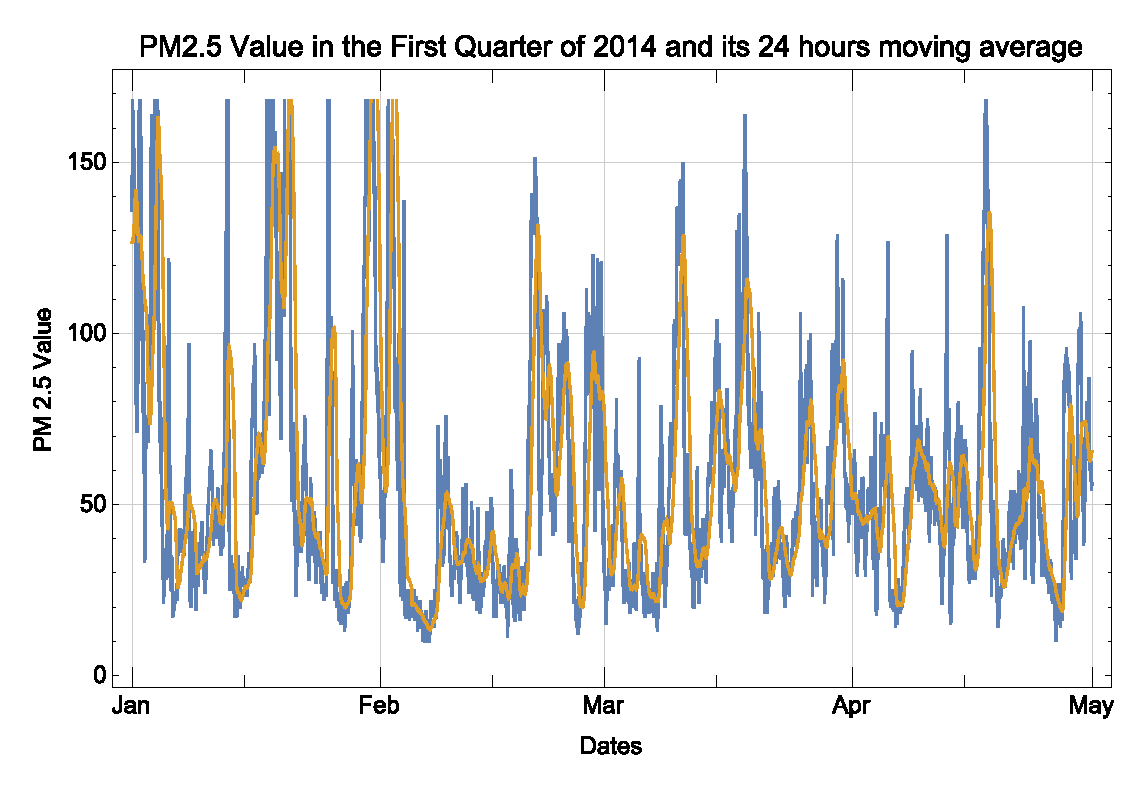
\includegraphics[width=0.50\textwidth]{PM25_MovingAverage.pdf}}
	\caption{Smooth Data using Moving Average}\label{fig:digit}
\end{figure}

After that, I run the Time Series Toolbox in \emph{Mathematica} [3] and work on the model selection part using AIC as criterion. Results are shown in the table below:

%%%Table 4: Model Selection: Top 5 Candidates
\begin{table}[h]
\begin{center}
\begin{threeparttable}
\begin{tabular}{c c c}
    \toprule
    \text{No} & \text{Candidate} & \text{AIC} \\ 
    \midrule
       1 & AR(1)  & 14651.5 \\
       2 & AR(2)   &  14651.9 \\ 
	3 & ARMA(2,1)   &  14653.2 \\ 
	4 & ARMA(1,1) &  14654.6 \\ 
	5 & MA(1) &  19831.6 \\ 
      \bottomrule
\end{tabular}
\end{threeparttable}
\end{center}
\caption{Model Selection: Top 5 Candidates}
\end{table}

You can see that the top four candidate models have very similar performs in terms of AIC, and later consideration, I pick ARMA(2,1) process and train a model based on it. Results are shown in Table 5. Finally, I use this process to estimate 3 days ahead $\text{PM}_{2.5}$ concentration index for the purpose of trend prediction and exhibit the results in Figure 4. 

%%%Table 5: ARMA(2,1) Model Results
\begin{table}[h]
\begin{center}
\begin{threeparttable}
\begin{tabular}{c c}
    \toprule
	\text{Parameters} & \text{Values} \\ 
    \midrule
       AR coefficient: $\phi_{1} $ & 0.642  \\
	AR coefficient: $\phi_{2} $  & 0.297  \\  	
	MA coefficient: $\theta_{1}$ & 0.269  \\ 
	White noise Variance: $\sigma^{2}$ & 158.7 \\ 
      \bottomrule
\end{tabular}
\end{threeparttable}
\end{center}
\caption{ARMA(2,1) Model Results}
\end{table}

%%%Figure 4: Trend Prediction using ARMA model
\begin{figure}[htbp]
	\centerline{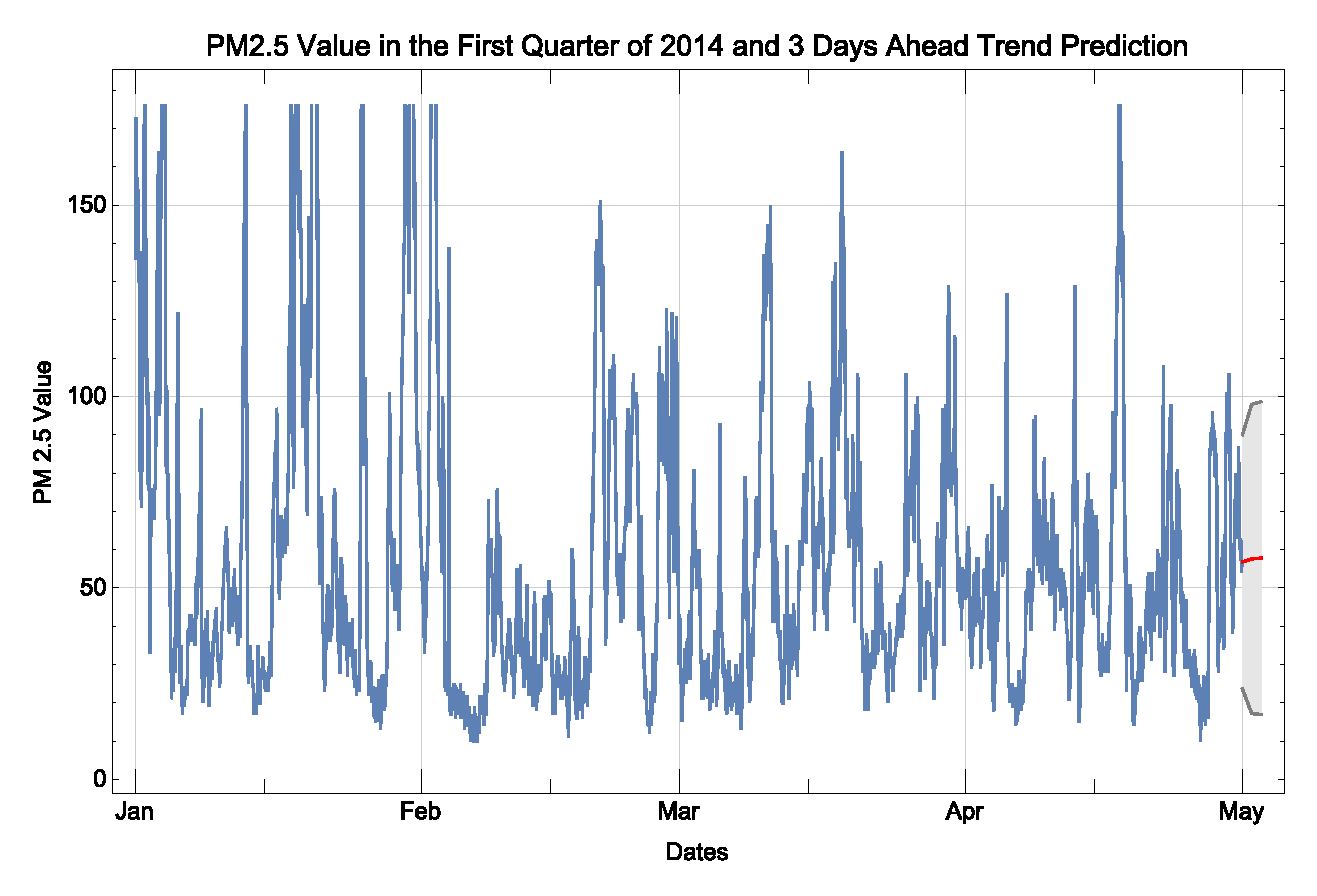
\includegraphics[width=0.50\textwidth]{PM25_ARMATrendPrediction.pdf}}
	\caption{Trend Prediction using ARMA model.}\label{fig:digit}
\end{figure}

The rightmost red curve in Figure 4 is the prediction trend (as well as values). The grey area are the 5\% $\sim$ 95\% confidence interval. 
Although this simple model successfully predict the trend during the period of May 1st to May 3rd, the confidence interval covers a huge area and thus tend to be less useful. You can also observe this drawback in Table 5 -- the White noise Variance $\sigma^{2}$ is extremely high. Besides, the ARMA model inclines to give a conservative prediction, and thus the forecast values looks like a straight line. 

Through analysis of the poor performance of ARMA model, we understand the importance of using a model with ``hidden states''. After making some further surveys, I resort another two models -- Stochastic Volatility Model and Stock-Watson Model.   

%Experiment II: Stochastic Volatility Model
\section{Experiment II: Stochastic Volatility Model}
Stochastic Volatility (SV) Model [4][5][6] is a non-linear state-space model. The intrinsic feature of the SV model is that each observation $y_{t}$ is assumed to have its ``own'' contemporaneous variance $e^{h_{t}}$. The SV model can thus be conveniently expressed in hierarchical form. In its center parameterization, it's given through
$$  y_{t} ~ | ~ h_{t}  \sim  N\left(0, exp ~ ( h_{t} ) \right) $$
$$  h_{t} ~ | ~ h_{t+1} , \mu, \phi, \sigma_{\eta}  \sim  N\left( \mu + \phi (h_{t-1} - \mu), \sigma_{\eta}^{2}  \right)$$
$$  h_{0} ~ | ~  \mu, \phi, \sigma_{\eta}  \sim  N\left( \mu ,  \sigma_{\eta}^{2} / (1 - \phi^{2})  \right)$$

\noindent where $\mu$ is the level of log-variance, $\phi$ is the persistence of log-variance, and $\sigma_{\eta}$ is the volatility of log-variance.

There are several important points we should notice in SV model. First, the mean of observation sequence $\{ Y_{t} \}$ should be zero, as shown in former equation one. As a result, if the raw dataset does not satisfy this restriction ( which is the case in this project as the mean of $\text{PM}_{2.5}$ values is non-zero ), we should manually convert it into the sequence we want. In order to achieve this, I first calculate the logarithm of $\text{PM}_{2.5}$ values, and then demean the difference of two continuous values. After this preprocessing step, We can get a time series satisfy the requirements of SV model.

The second characteristic of SV model is the existence of static parameters, namely $\mu$, $\phi$ and $\sigma_{\eta}$. This is very different from the Stock-Watson Model discussed in next section. In order to make inference on these parameters, I resort to the full Bayesian framework and utilizes Markov Chain Monte Carlo (MCMC) samplers. 

The level $\mu \in \mathbb{R}$ is equipped with the usual normal prior $\mu \sim N(b_{\mu}, B_{\mu})$. I set $b_{\mu} = 0 $ and $B_{\mu} = 100$ for non-informative prior. For the persistence parameter $\phi \in (-1, 1)$, I choose $(\phi + 1) /2  \sim \mathcal{B}(a_{0}, b_{0})$, implying 

$$ p(\phi) = \frac{1}{2\mathcal{B}(a_{0},b_{0})} \left( \frac{1+\phi}{2} \right)^{a_{0}-1} \left( \frac{1-\phi}{2} \right)^{b_{0}-1}  $$

\noindent where $\mathcal{B}(a_{0},b_{0})$ denotes the beta function, and I choose the hyperparameters $a_{0} = 20, b_{0} = 1.1$. Finally, for the volatility of log-variance $\sigma_{\eta} \in \mathbb{R}^{+}$, we choose $\sigma_{\eta}^{2} \sim \mathcal{B}_{\sigma_{\eta}} \times \chi_{1}^{2} = \mathbb{G}(1/2 , 1/2\mathcal{B}_{\sigma_{\eta}})  $. The hyperparameter $\mathcal{B}_{\sigma_{\eta}}$ is chosen to be $0.1$, which is of minor influence in empirical applications. 

The aggregated results including posterior distribution of three parameters and the predicted volatility are shown in Table 6 and Figure 5.  

%%%Table 6: Posterior draws of parameters
\begin{table}[h]
\begin{center}
\begin{threeparttable}
\begin{tabular}{c c c c c}
    \toprule
	\text{Parameter} & \text{Mean} & \text{sd} & \text{5\%} & \text{95\%} \\ 
    \midrule
       $\mu$ & -3.69  & 0.173 & -3.973 & -3.41 \\
	$\phi$ & 0.92 & 0.021 & 0.888 & 0.95 \\
	$\sigma_{\eta} $ & 0.37 & 0.049 & 0.088 & 0.21 \\
      \bottomrule
\end{tabular}
\end{threeparttable}
\end{center}
\caption{Posterior draws of hyperparameters}
\end{table}

%%%Figure 5: Result of SV model on $\text{PM}_{2.5} dataset
\begin{figure}[htbp]
	\centerline{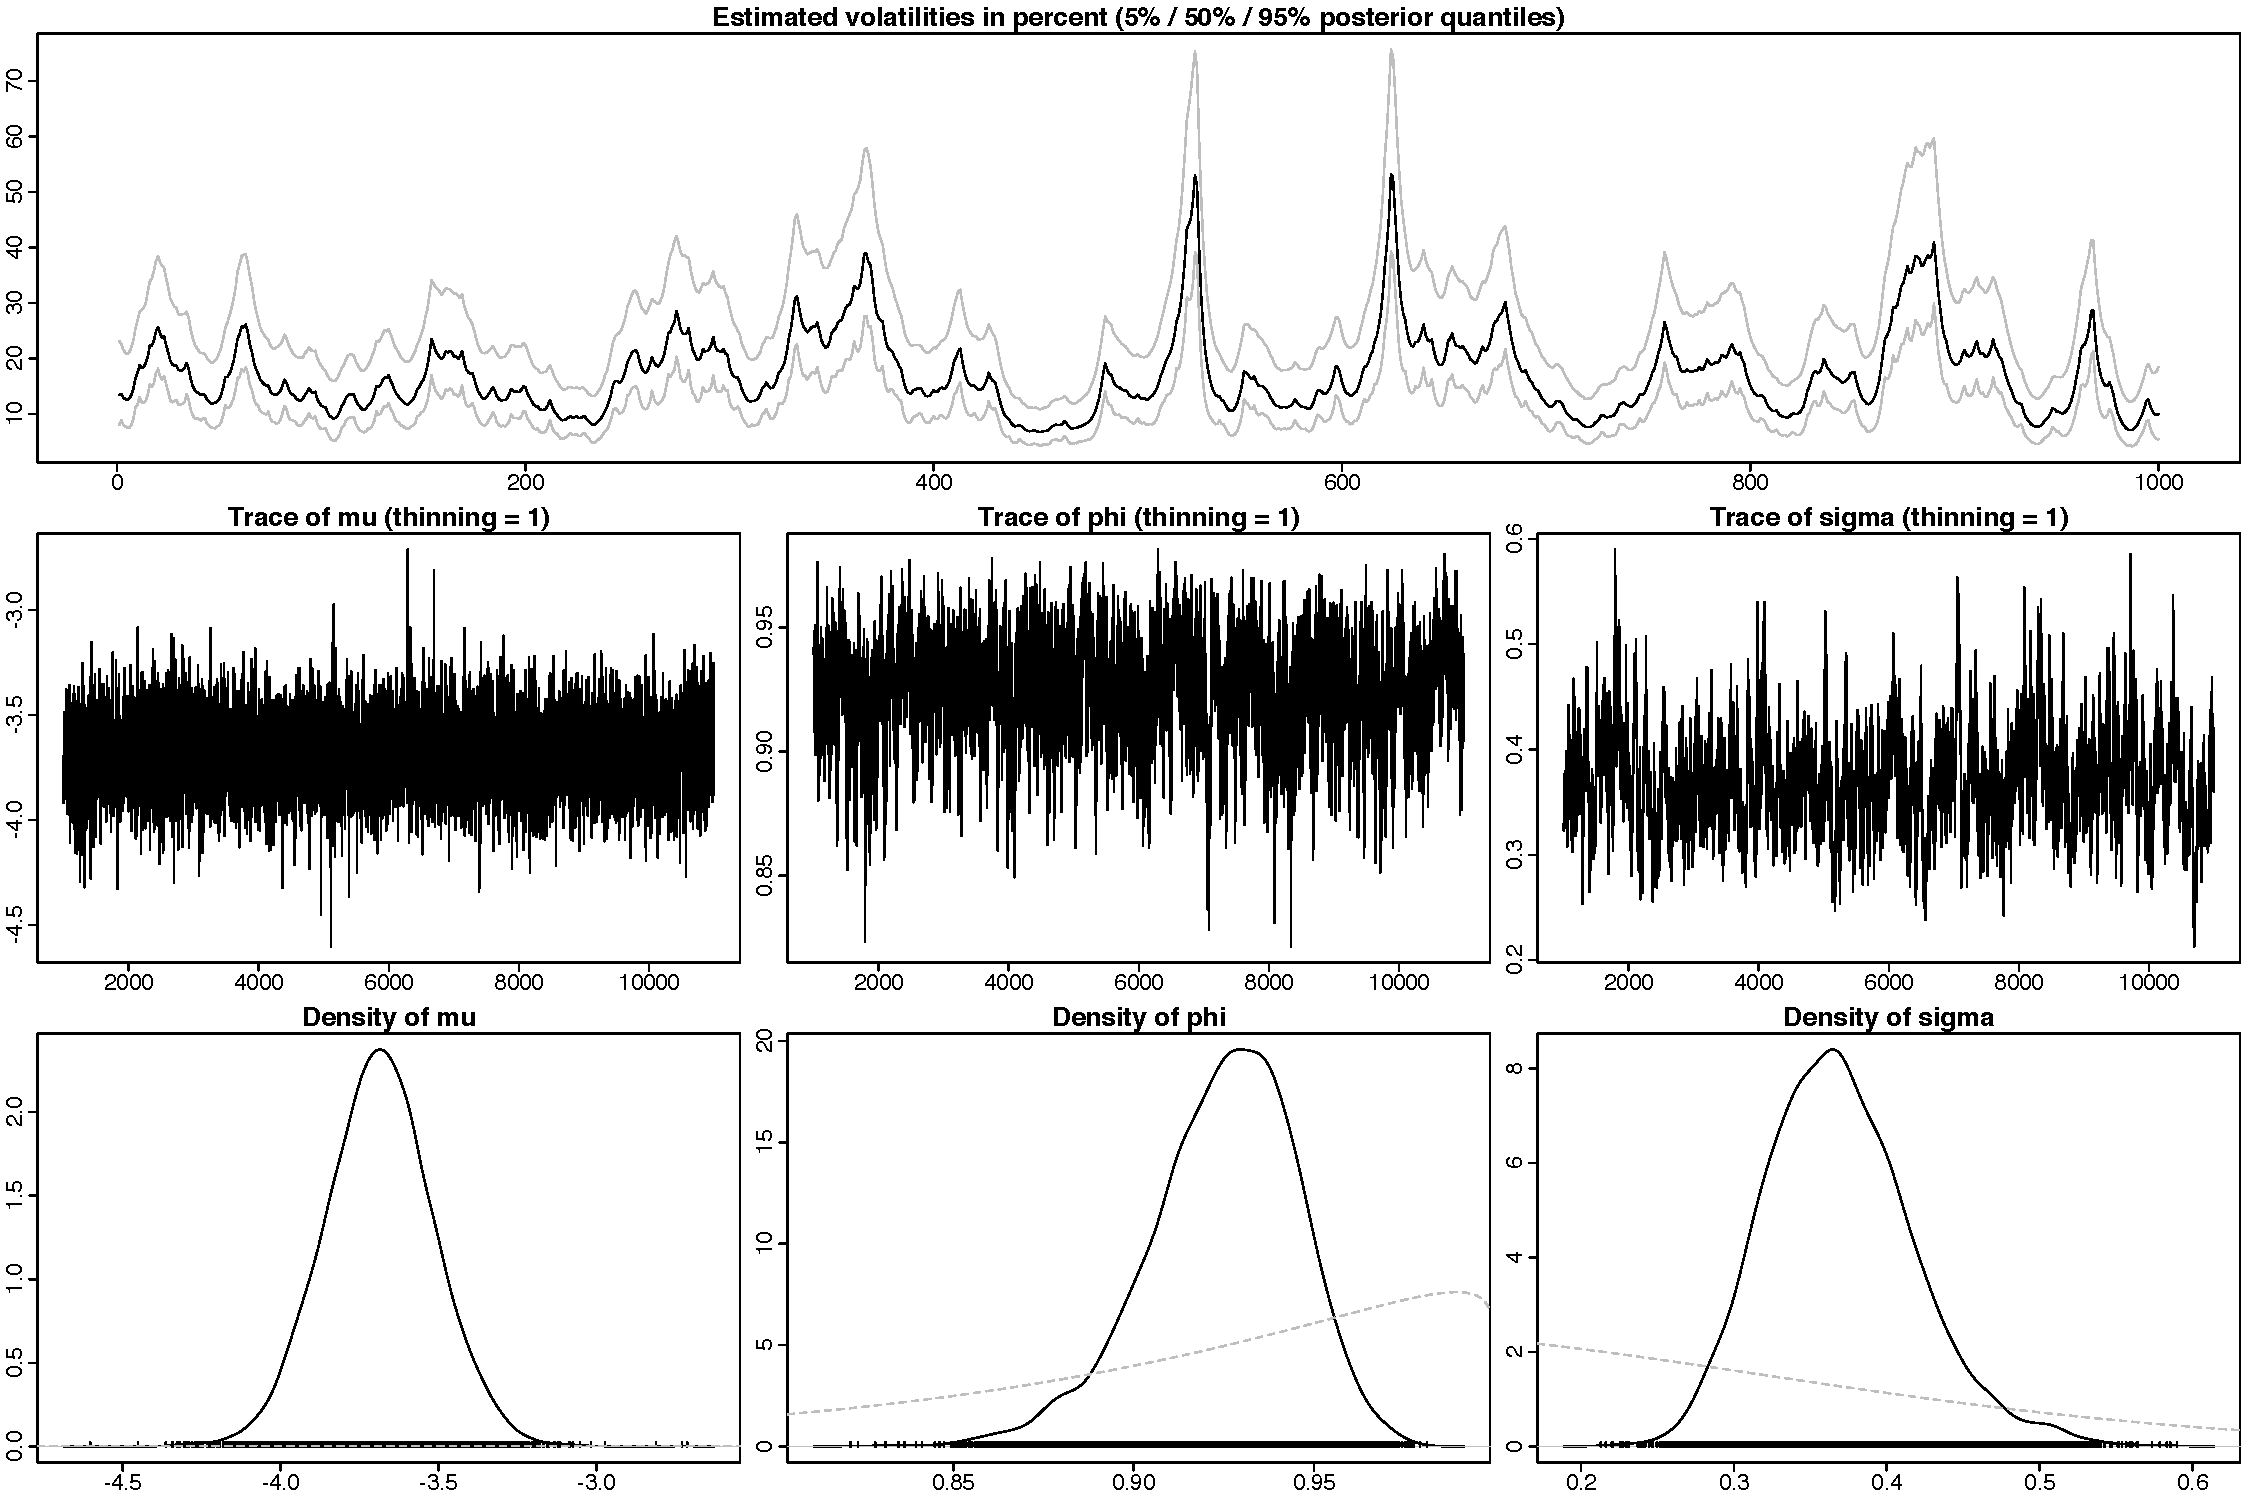
\includegraphics[width=0.50\textwidth]{PM25_SV.pdf}}
	\caption{Result of SV model on $\text{PM}_{2.5}$ dataset}\label{fig:digit}
\end{figure}

Finally, we should notice that all hyperparameters, estimated latent states and predicted volatility are in the ``Hidden State Space''. Thus, SV model provides an excellent tool to conduct hidden factors prediction, however, it's not suitable for making $\text{PM}_{2.5}$ Trend or Value Prediction. In future work, I think I could use SV model to extract some latent features of $\text{PM}_{2.5}$ concentration index. For example, I can use the predicted volatility as the measure of ``aggressiveness'' of one-step or multiple-steps prediction. 

%Experiment III: Stock-Watson Model
\section{Experiment III: Stock-Watson Model}
Stock-Waston (SW) Model is recently proposed in [7], and its brief explanation can be found in Section 2.5.7 of [5]. It is a time-varying random walk plus local level model. 
$$ \pi_{n} = \mathbf{x}_{1,n} + \varepsilon_{n}, \qquad \varepsilon_{n} \sim N(0, \text{exp}(\mathbf{x}_{2,n}) ) $$
$$ \mathbf{x}_{1,n+1} = \mathbf{x}_{1,n} + \eta_{n}, \qquad \eta_{n} \sim N(0, \text{exp}(\mathbf{x}_{3,n}) ) $$
$$ \mathbf{x}_{2,n+1} = \mathbf{x}_{2,n} + \omega_{1,n}, \qquad \omega_{1,n} \sim N(0, 0.2)  $$
$$ \mathbf{x}_{3,n+1} = \mathbf{x}_{3,n} + \omega_{2,n}, \qquad \omega_{2,n} \sim N(0, 0.2)  $$
\noindent where $\mathbf{x}_{1,n}$ in this project is the unobserved time-varying mean of $\text{PM}_{2.5}$ and $\mathbf{x}_{i,n}$ for $i = 2, 3$ are unobserved log-variances. Conditional on the log-variance $\mathbf{x}_{2,n}$ and $\mathbf{x}_{3,n}$, the remaining model is a linear, Gaussian state space model, and thus it can then be calculated exactly by the Kalman Filter. 

There are two appealing characters of this model. First, the introduction of $\mathbf{x}_{1,n}$ enables the observation $\pi_{n}$ to possess non-zero mean. Second, there are no static parameters that need to estimated due to the special structure of this model. We can fit this model using Rao-Blackwellized particle filter technique. I plot the one step ahead prediction in Figure 6. 

%%%Figure 6: One Step Ahead Prediction Using Stack-Watson Model
\begin{figure}[htbp]
	\centerline{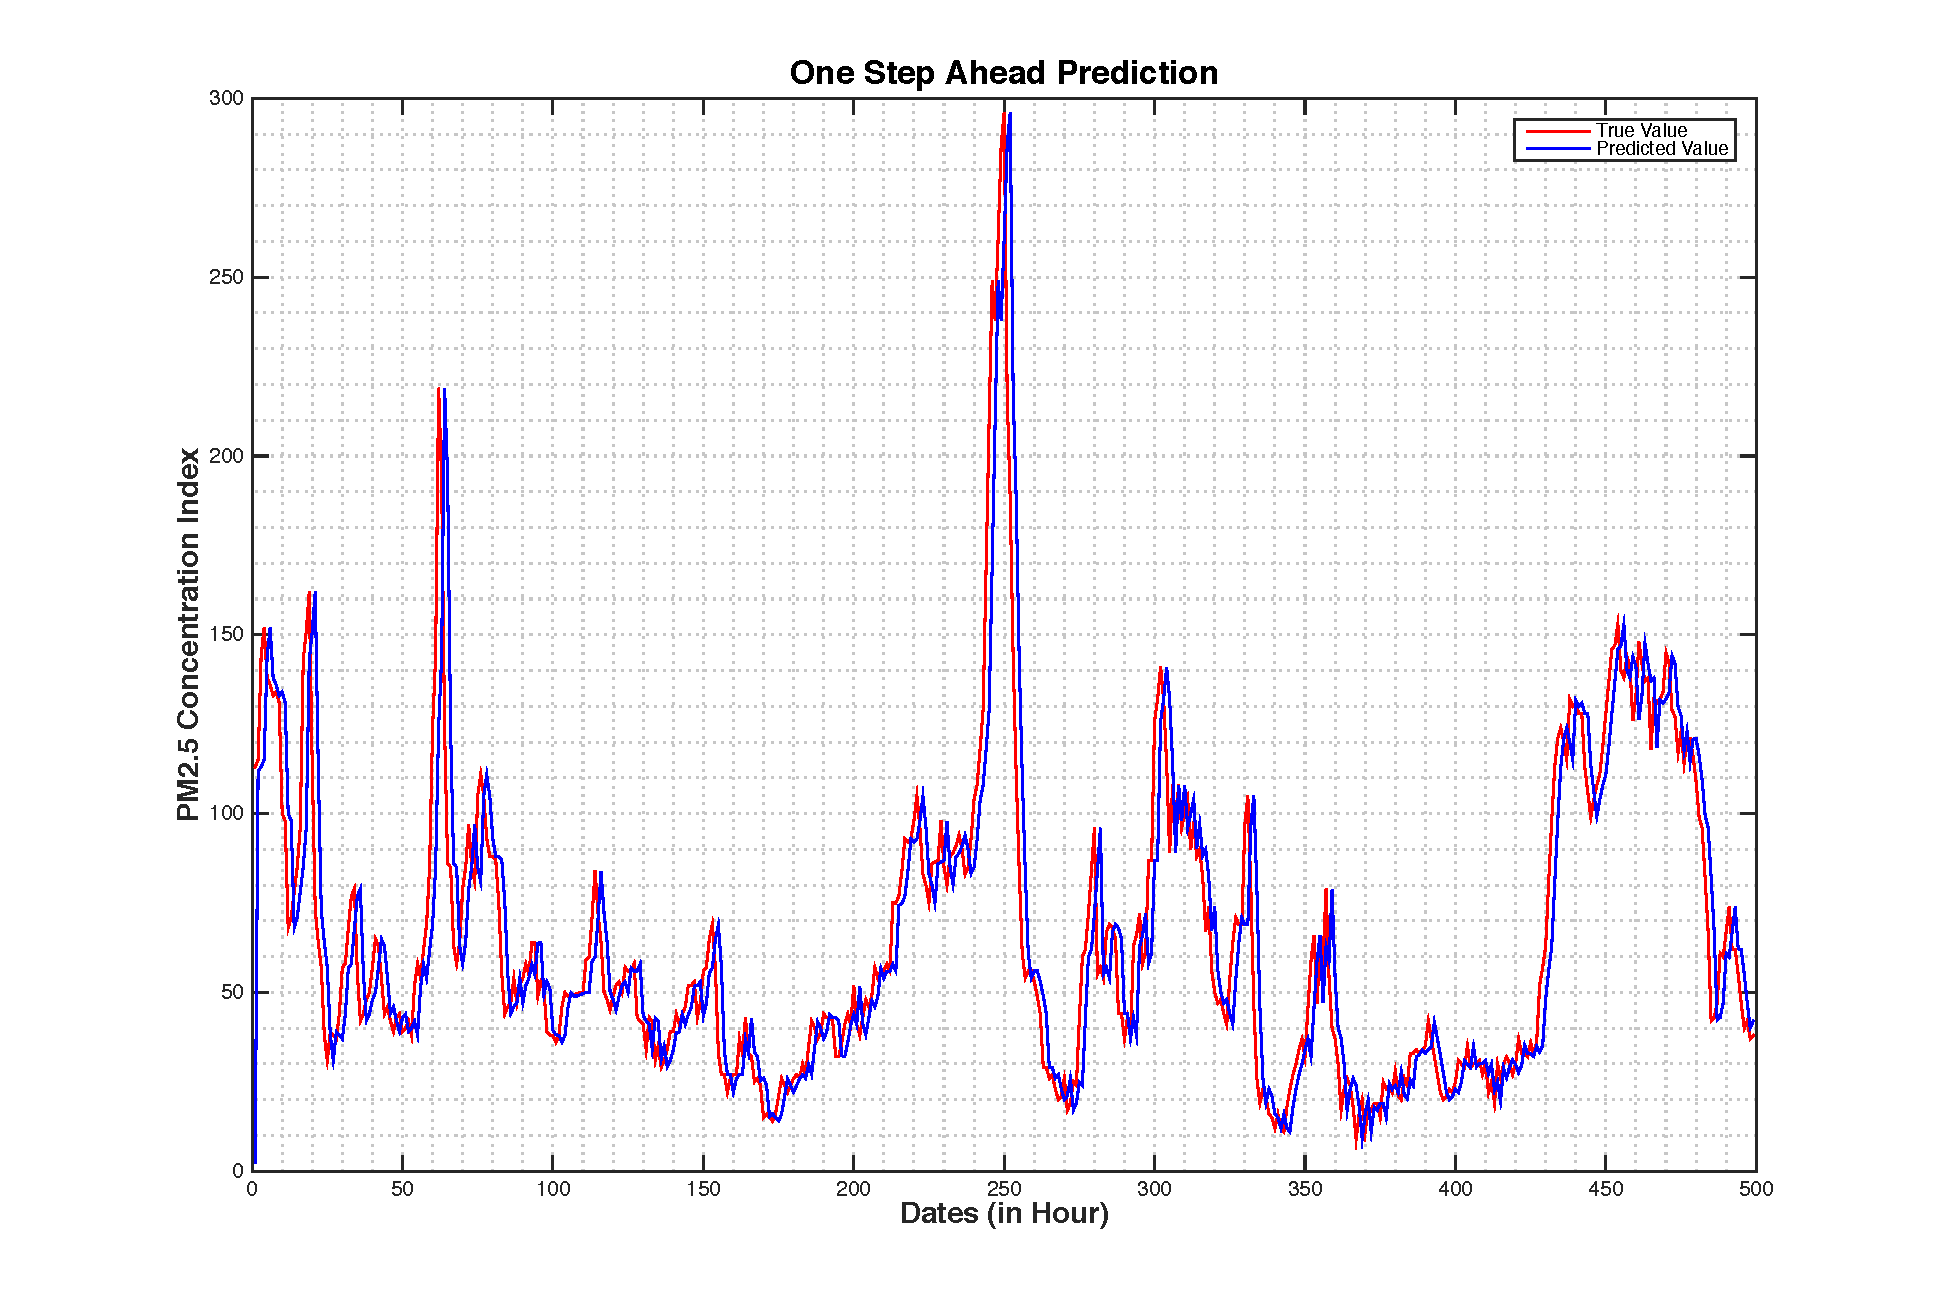
\includegraphics[width=0.50\textwidth]{PM25_onestep.pdf}}
	\caption{One Step Ahead Prediction Using Stack-Watson Model}\label{fig:digit}
\end{figure}

When viewed in high level, this model seems to fit the trend and values of $\text{PM}_{2.5}$ concentration index. However, there are several major drawbacks. First, this model requires the true observation every time when it makes further prediction, and thus it can only make accurate one-step ahead prediction. Second, it presents sort of time-delay when making prediction. Actually, if we observed this results in detail, the average difference between true value and predicted value is 12.7463, which is not good enough. Despite of all these problems, Stock-Watson model is currently the most promising off-the-shelf method and serves as the foundation of an extended model discussed in the following section.

%Experiment III: Stock-Watson Model with External Information
\section{Experiment IV: Stock-Watson Model with External Information}
All above-mentioned models have a common problem, i.e., they failed to take consideration of external information. When talking about $\text{PM}_{2.5}$, people normally think of the weather data. Based on this intuition, I combine the prediction output by SW model with the external weather information. To be more specific, every time we get a output from SW model, instead of using this value as the prediction directly, I view it as a part of input features which also contains the weather information such as temperature, pressure, humidity, windspeed and precipitation rate. Our goal is to output the final prediction based on the input feature vector. This is a regression problem! In order to solve this problem, I adopt a time series neural network with the architecture shown in Figure 7.

%%%Figure 7: Nonlinear Autoregressive with External Input (NARX) architecture 
\begin{figure}[htbp]
	\centerline{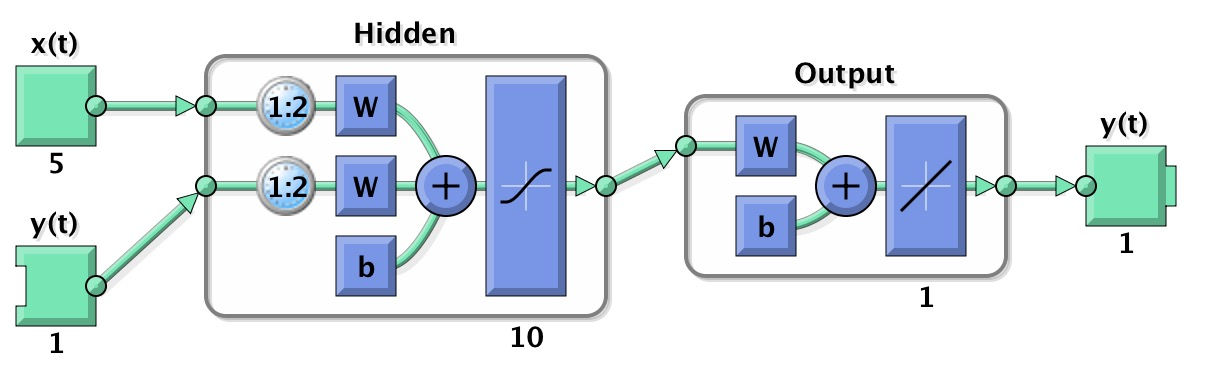
\includegraphics[width=0.45\textwidth]{PM25_NN_arch.jpg}}
	\caption{Nonlinear Autoregressive with External Input (NARX) architecture }\label{fig:digit}
\end{figure}

Using the first 500 hourly $\text{PM}_{2.5}$ concentration indexes of Shanghai in Year 2012, I train this neural network with 10 hidden units and 2 units time delays. In addition, I adopt the Bayesian Regularization in the training process to deal with overfitting problem. Results are shown in Figure 8 and Figure 9. 

%%%Figure 8: Response Plot of (NARX) neural network
\begin{figure}[htbp]
	\centerline{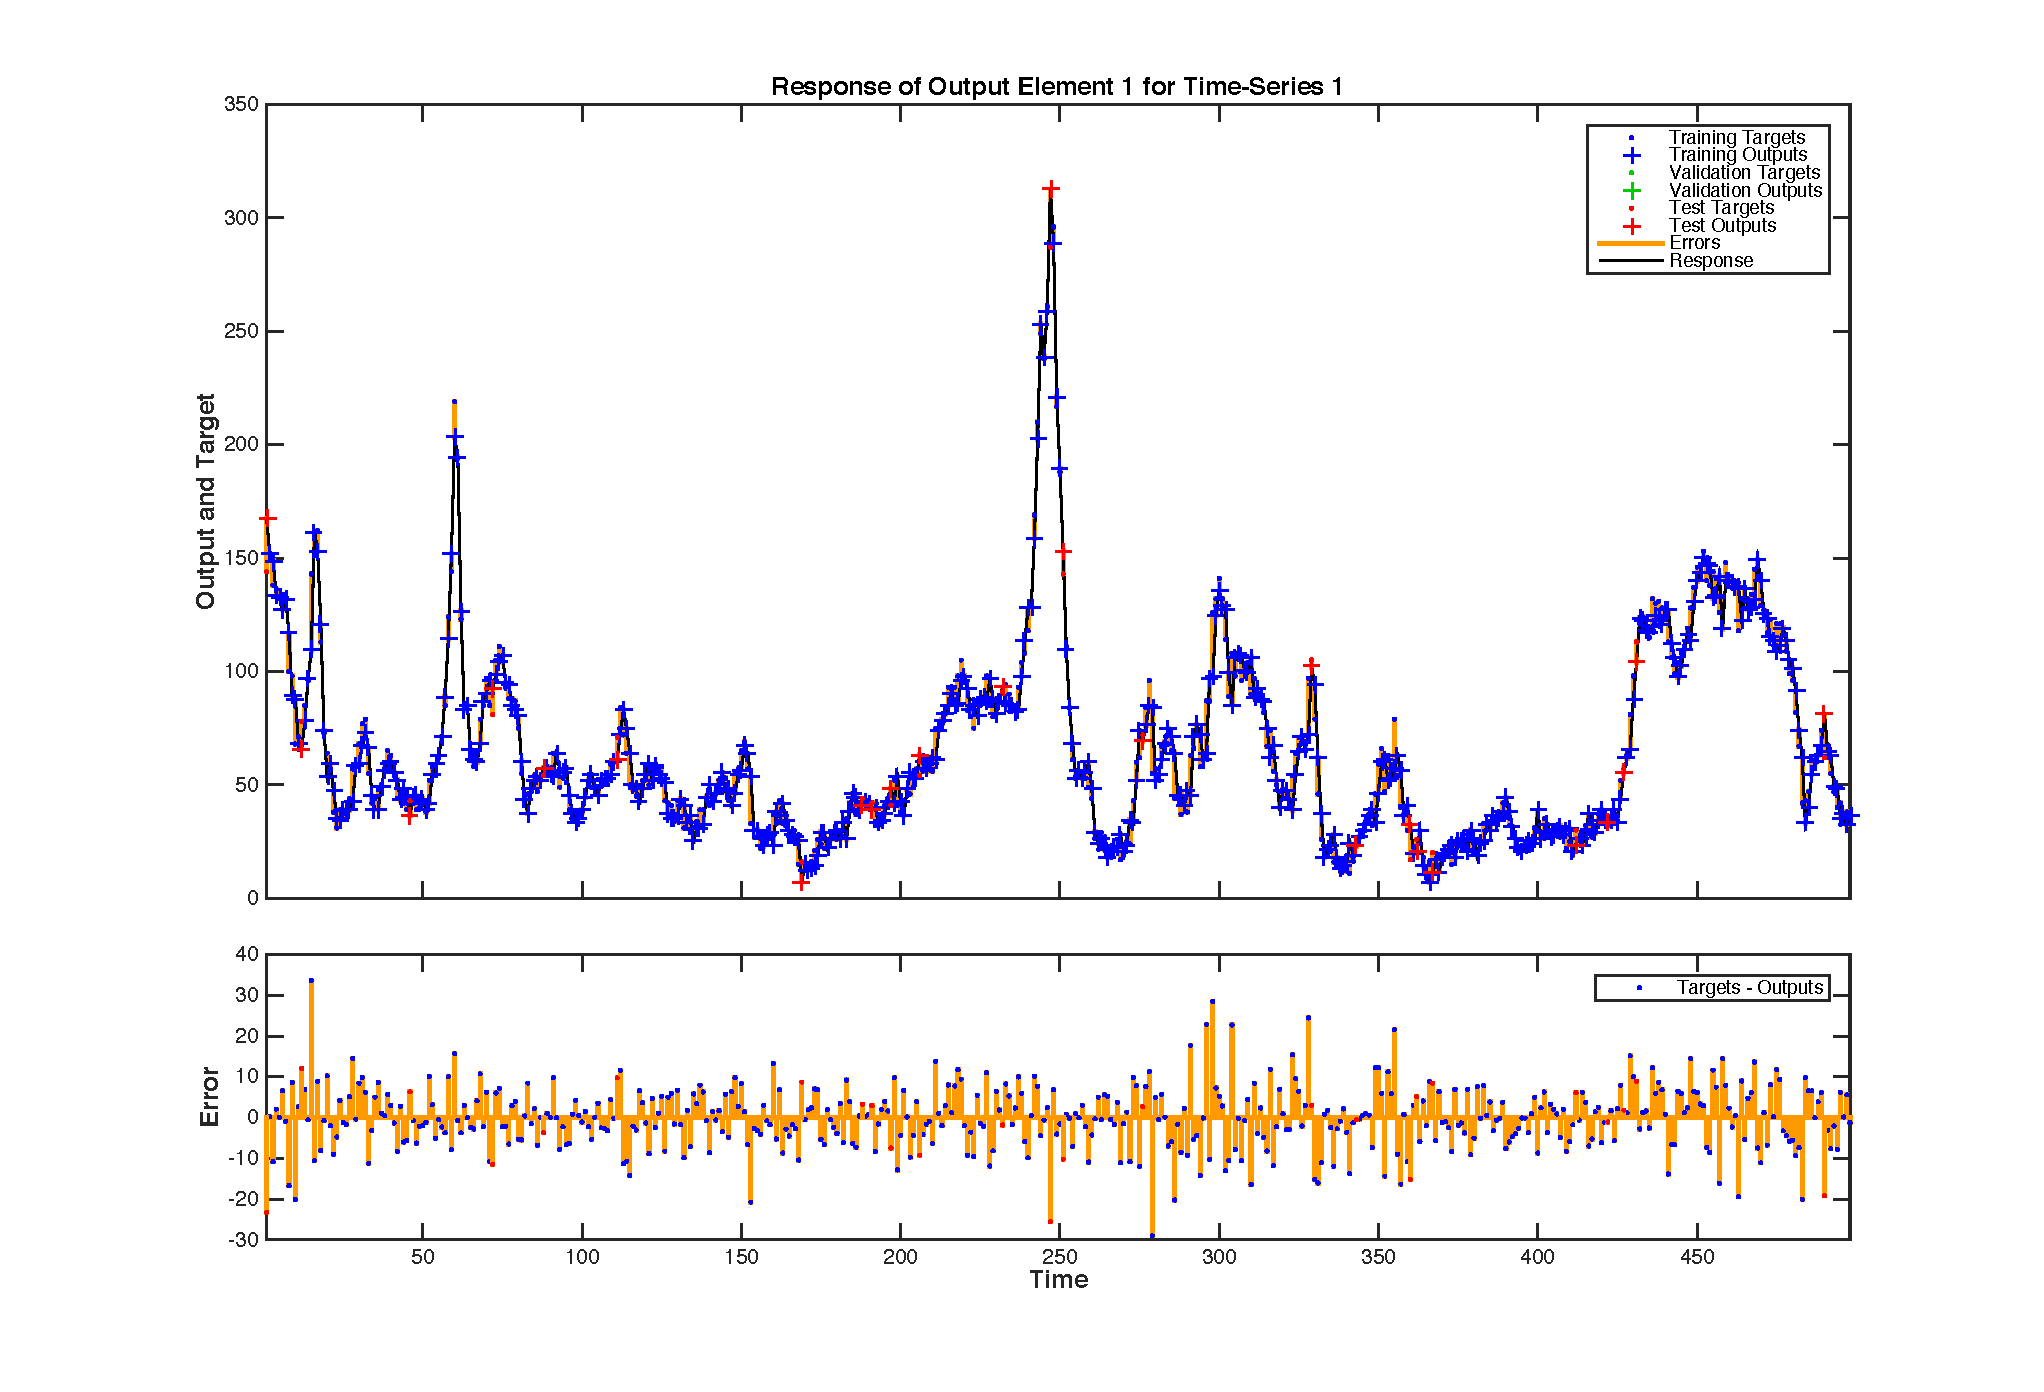
\includegraphics[width=0.60\textwidth]{PM25_h10d2_tsResponse.pdf}}
	\caption{Response Plot of (NARX) neural network }\label{fig:digit}
\end{figure}

As you can see, the error in most of time stamps belongs to range $[ -7, +8]$. The MSE reduces to approximately 50, when using this method. 

%%%Figure 9: Error Histogram of (NARX) neural network 
\begin{figure}[htbp]
	\centerline{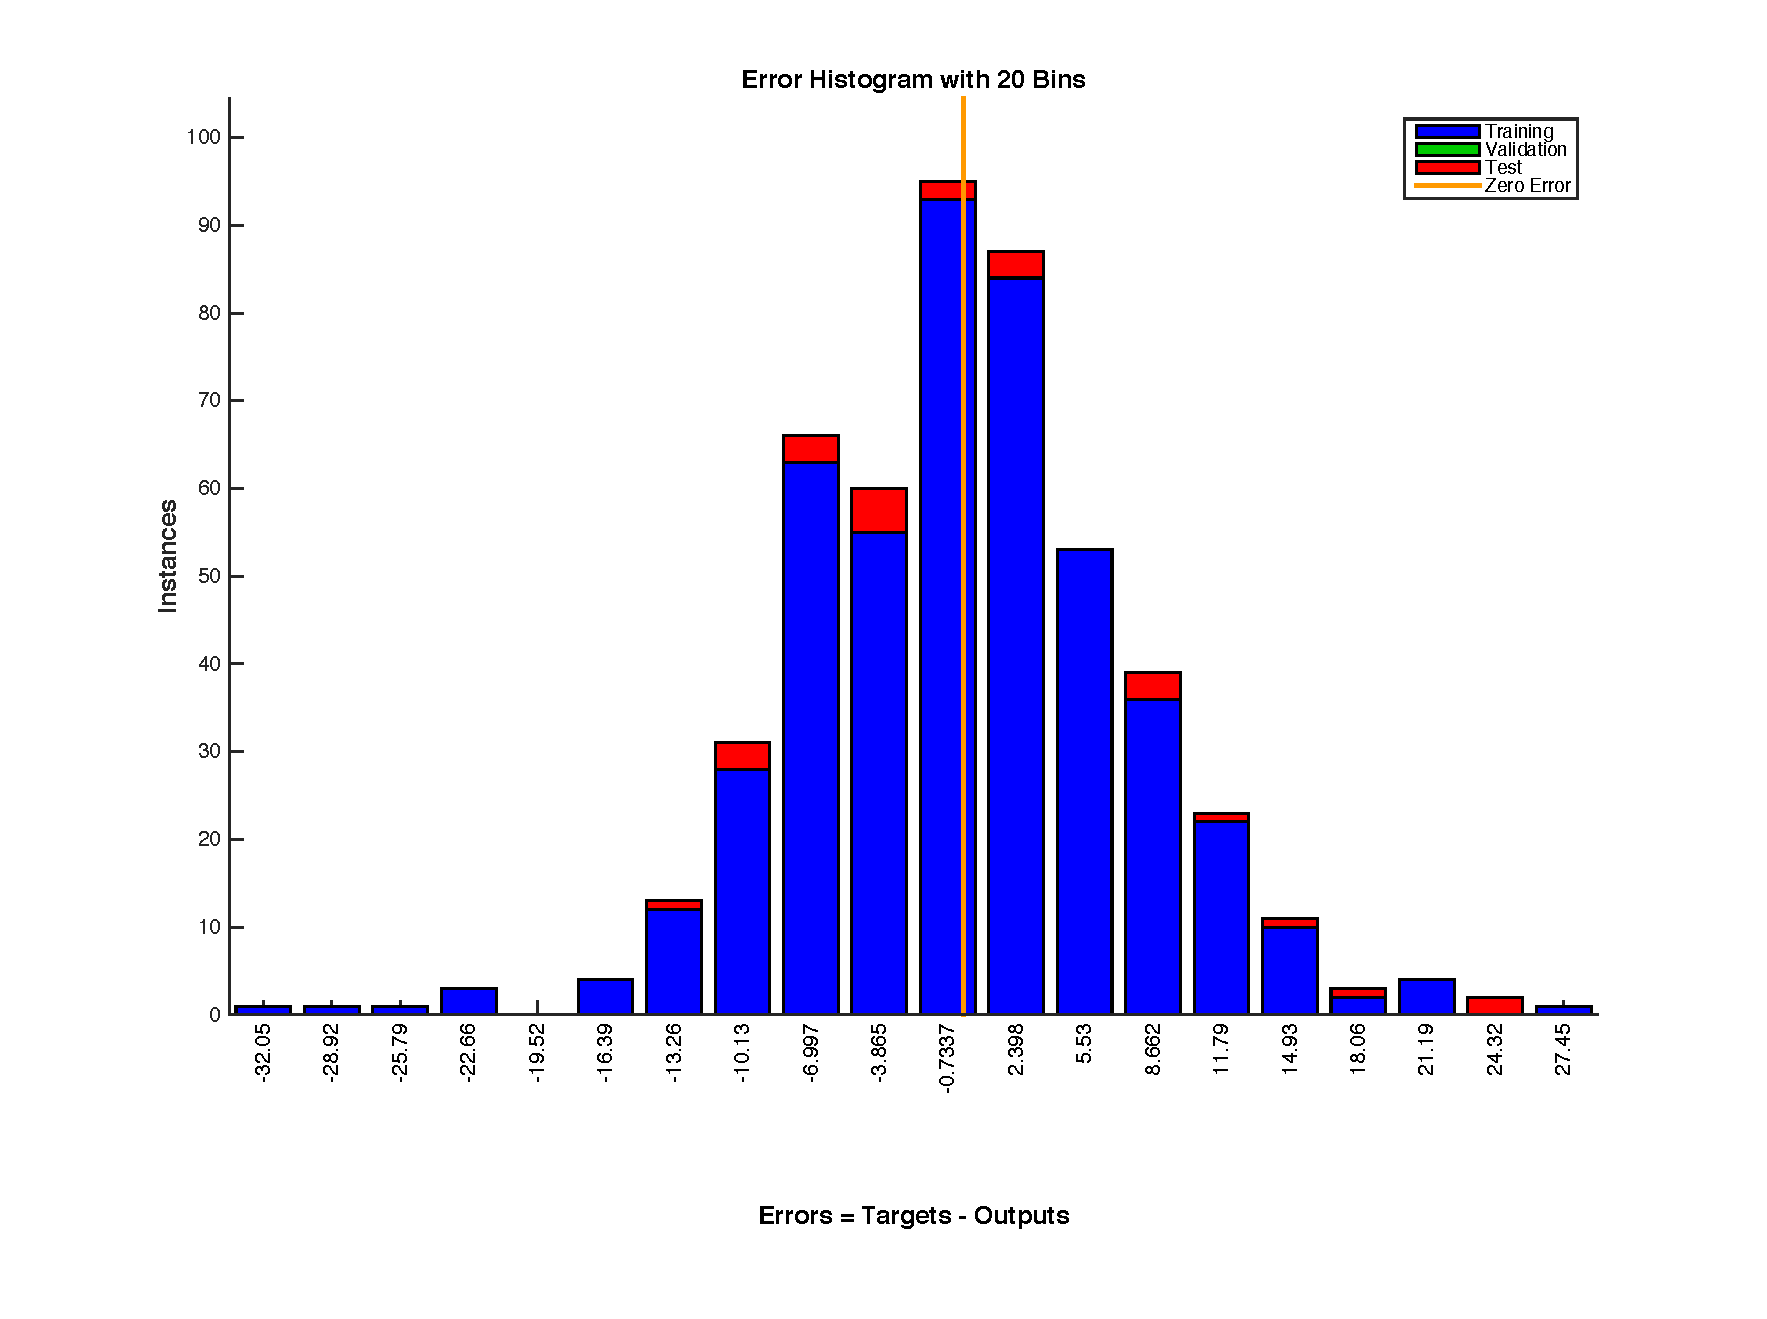
\includegraphics[width=0.60\textwidth]{PM25_h10d2_tsErrorHist.pdf}}
	\caption{Error Histogram of (NARX) neural network }\label{fig:digit}
\end{figure}

Finally, I will compare this method with another two methods through solving multi-step prediction problems. I train the models with first 500 hours day points and evaluate its performance using six steps ahead prediction. As mentioned below, the original version SW model is not able to make multi-step prediction, so I modify it by letting the next ``true'' observation equal to the last prediction. Results are shown in Figure 10.  

%%%Figure 10: Predicted $\text{PM}_{2.5}$ Values using Three Different Methods
\begin{figure}[htbp]
	\centerline{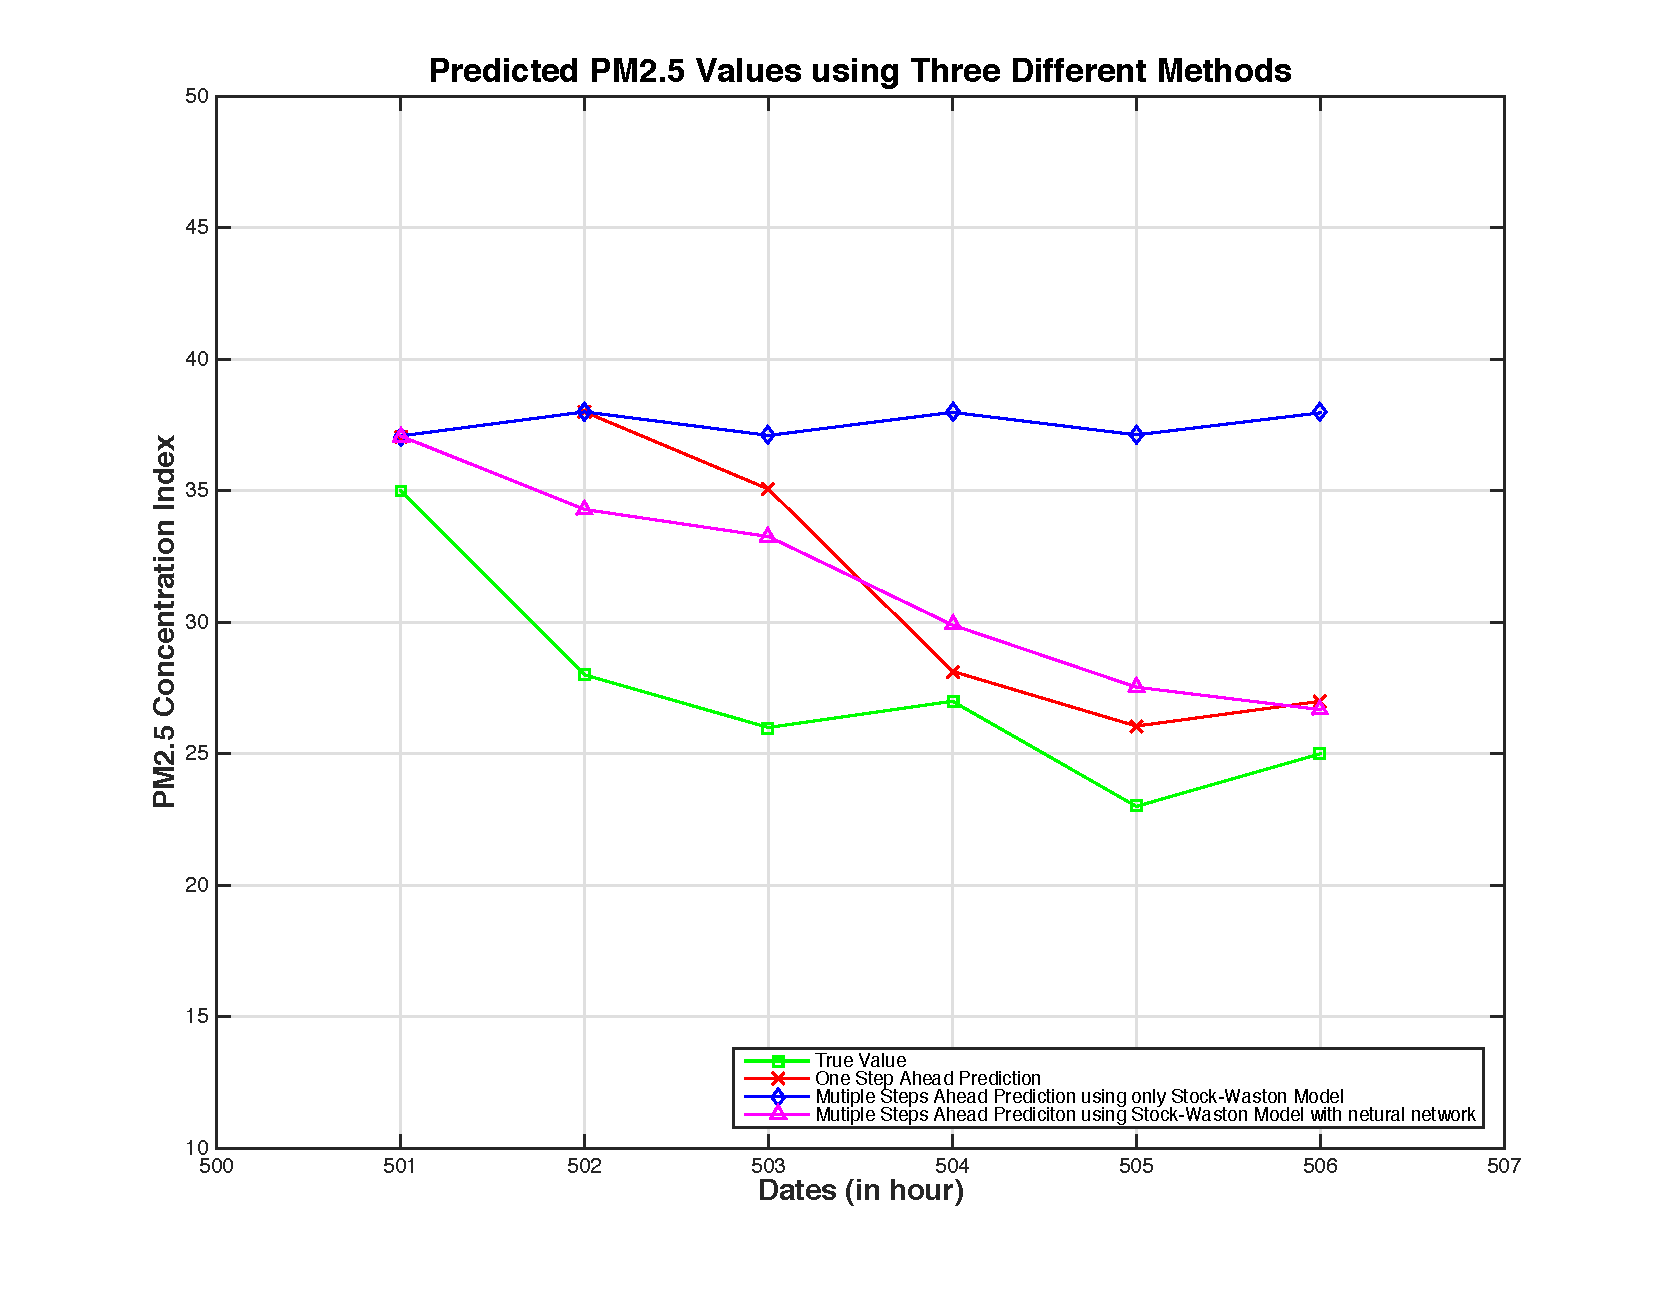
\includegraphics[width=0.50\textwidth]{PM25_methods.pdf}}
	\caption{Predicted $\text{PM}_{2.5}$ Values using Three Different Methods }\label{fig:digit}
\end{figure}

You can see the true value of $\text{PM}_{2.5}$ is decreasing, while the multiple steps ahead predictions using only SW model remain basically the same. This is because SW model adjust its predictions by comparing them with the true observation values, however, in order to achieve multi-step prediction, we let the ``true'' observation to be same with last prediction and thus SW model loses its ability to recover from bad prediction. The modified version of SW model overcomes this problem by using external information, and achieves a better performance.

%Future Works \& Conclusion
\section{Conclusion \& Future Works }
There are several places I can further improve in future. First, I should clean my original dataset more carefully. In this project, I simply adopt the first-order interpolation method which only works when the number of missing data in a row is not very high. However, after a more detailed observation of raw dataset, I find sometimes there will be over 30 continuous missing data. This phenomenon requires more careful data pre-processing. 

Second, I should put more effects on the latent variables. These hidden factors not only serves as a way to improve the prediction accuracy, which is basically this report focused on, but also should be considered as the fundamental reasons leading to the $\text{PM}_{2.5}$ concentration index trend. As mentioned in ``Experiment II: Stochastic Volatility Model'', I could use the SV model as a method to extract hidden features of observable $\text{PM}_{2.5}$ values. 

Finally, I should develop my own model to make $\text{PM}_{2.5}$ concentration index prediction, based on this problem's own characteristics. In this report, I briefly talk about one simple modification of Stock-Watson Model and show its corresponding performance improvement. Through further analyze on this problem and more discussion with TAs, I will figure out a more suitable model to deal with it. 

\section{Reference}
\noindent [1]. U.S. Department of State.

\noindent [2]. Air Quality Data Files. 

\noindent [3]. Mathematica Time Series Toolbox

\noindent [4]. Liu, Jun S. \emph{Monte Carlo strategies in scientific computing}. Springer Science \& Business Media, 2008.

\noindent [5]. Creal, Drew.``A survey of sequential Monte Carlo methods for economics and finance.'' \emph{Econometric Reviews} 31.3 (2012): 245-296.

\noindent [6]. Kastner, Gregor. ``Dealing with stochastic volatility in time series using the R package stochvol." \emph{Journal of Statistical Software}.

\noindent [7]. Stock, James H. and Mark W. Watson. ``Why Has U.S. Inflation Become Harder to Forecast?" \emph{Journal of Money, Credit and Banking} 39, s1 (2007): 13 - 33s

\noindent [8]. Matlab Neural Network Toolbox

\end{document}
